\chapter{The models}
In this chapter we discuss several neural network classifiers and their results on our dataset.
\section{Baseline model}
We decided to start with an adaptation of the \textit{optimal} model's architecture outlined in \cite{blackardDean} and reported in Figure \ref{fig:baselinemodel}. The model is made of 51 input nodes, 120 hidden nodes and seven output nodes (symbolized as 51-120-7) where each layer is fully connected. Both the hidden and output layers utilized the logistic (sigmoid) activation functions:
$$
\sigma(a) = \frac{1}{1 + e^{-a}}
$$
Given the training set size, we picked SGD (Stochastic Gradient Descent) as loss function optimizer, while the loss function is the classic MSE (Mean Squared Error, as in \cite{blackardDean}):
\begin{equation}
\text{MSE} = \frac{1}{n}\sum_{i=1}^{n}(Y_i - Y^{*}_{i})^2
\end{equation}
where $Y_i$ is the vector of the true values of the target, $Y^{*}_{i}$ is the model's prediction and $n$ is the number of samples.
\begin{figure}
\centering
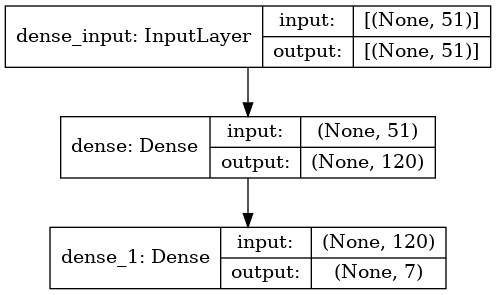
\includegraphics[width=0.7\textwidth]{./TeX_files/img/baselinemodel.png}
\caption{Baseline model diagram.}
\label{fig:baselinemodel}
\end{figure}
Setting the learning rate (LR) to $0.05$, the batch size to $128$ and the number of epochs to $200$ the classifier has been trained via a 10-fold cross-validation. The accuracy on the train set and the validation set is shown in Figure \ref{fig:baselinemodelacc} while the losses in Figure \ref{fig:baselinemodelloss}: to smooth the plots, the last metric value for each fold has been taken into account.
\begin{figure}
\centering
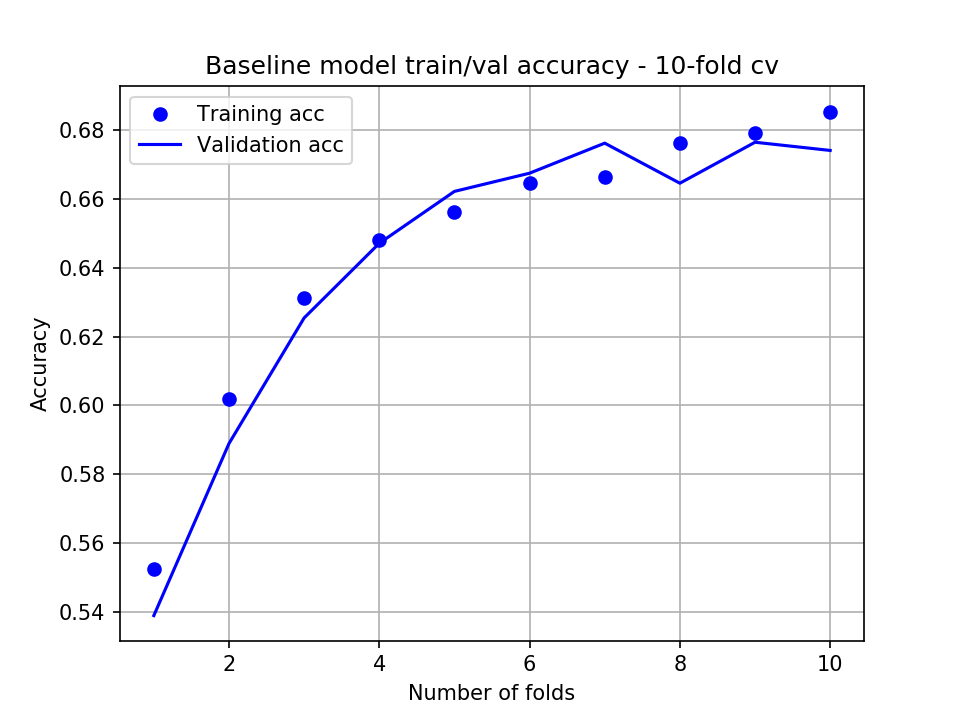
\includegraphics[width=0.7\textwidth]{./TeX_files/img/baselinemodelacc.png}
\caption{Baseline model accuracy.}
\label{fig:baselinemodelacc}
\end{figure}
\begin{figure}
\centering
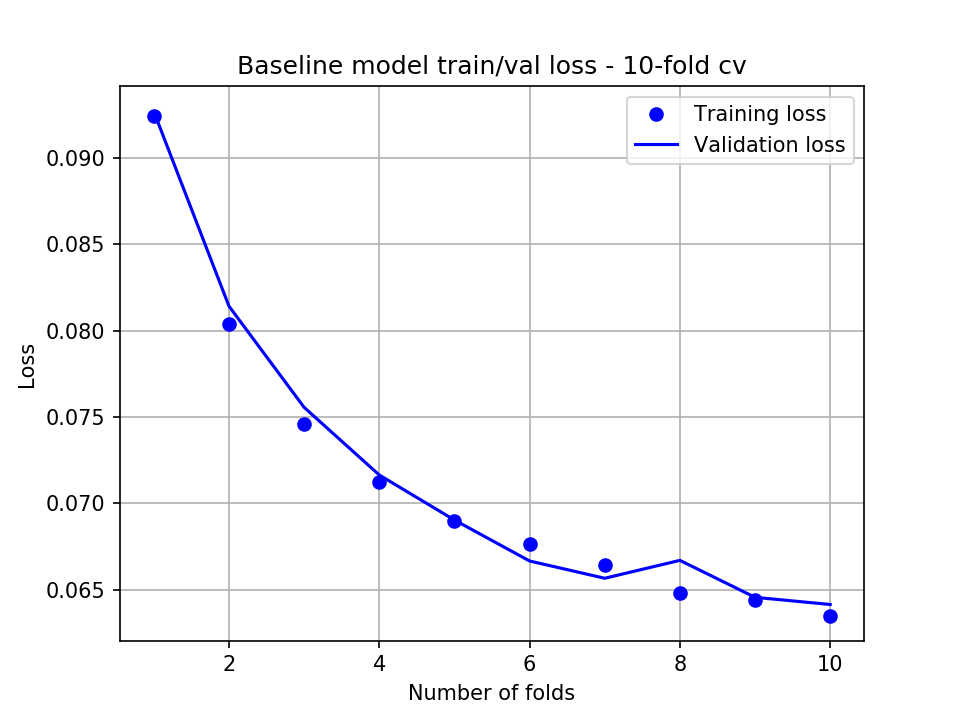
\includegraphics[width=0.7\textwidth]{./TeX_files/img/baselinemodelloss.png}
\caption{Baseline model losses.}
\label{fig:baselinemodelloss}
\end{figure}
Given the multi-class nature of the classification task, Figure \ref{fig:confmatheatmap} represent the heat-map rendering of the classification matrix to better convey the information regarding the correctly classified/misclassified samples: it is easy to notice that $532$ samples, of the total $587$ in the test set, belonging to the minority class (Cottonwood/Willow) are correctly classified; $5285$ are misclassified as the minority class but they belong to Ponderosa Pine. Moreover, a good amount of Spruce/Fir samples are correctly classified (this should be expected since this class is one of the majority classes). Other useful performance metrics for imbalanced class problems are precision (PRE), recall (REC) and F1-score (F1):
\begin{equation}
\begin{aligned}
\text{PRE} &= \frac{TP}{TP+FP} \\
\text{REC} &= \frac{TP}{FN+TP} \\
\text{F1} &= 2 \cdot \frac{\text{PRE} \cdot \text{REC}}{\text{PRE} + \text{REC}}
\end{aligned}
\end{equation}
where $TP$ stands for True Positive, $FP$ for False Positive and $FN$ for False Negative. According to these definitions, Table \ref{tab:classificationrep} summarise each metric for each class. FARE ESEMPIO di weighted avg.
\begin{figure}
\centering
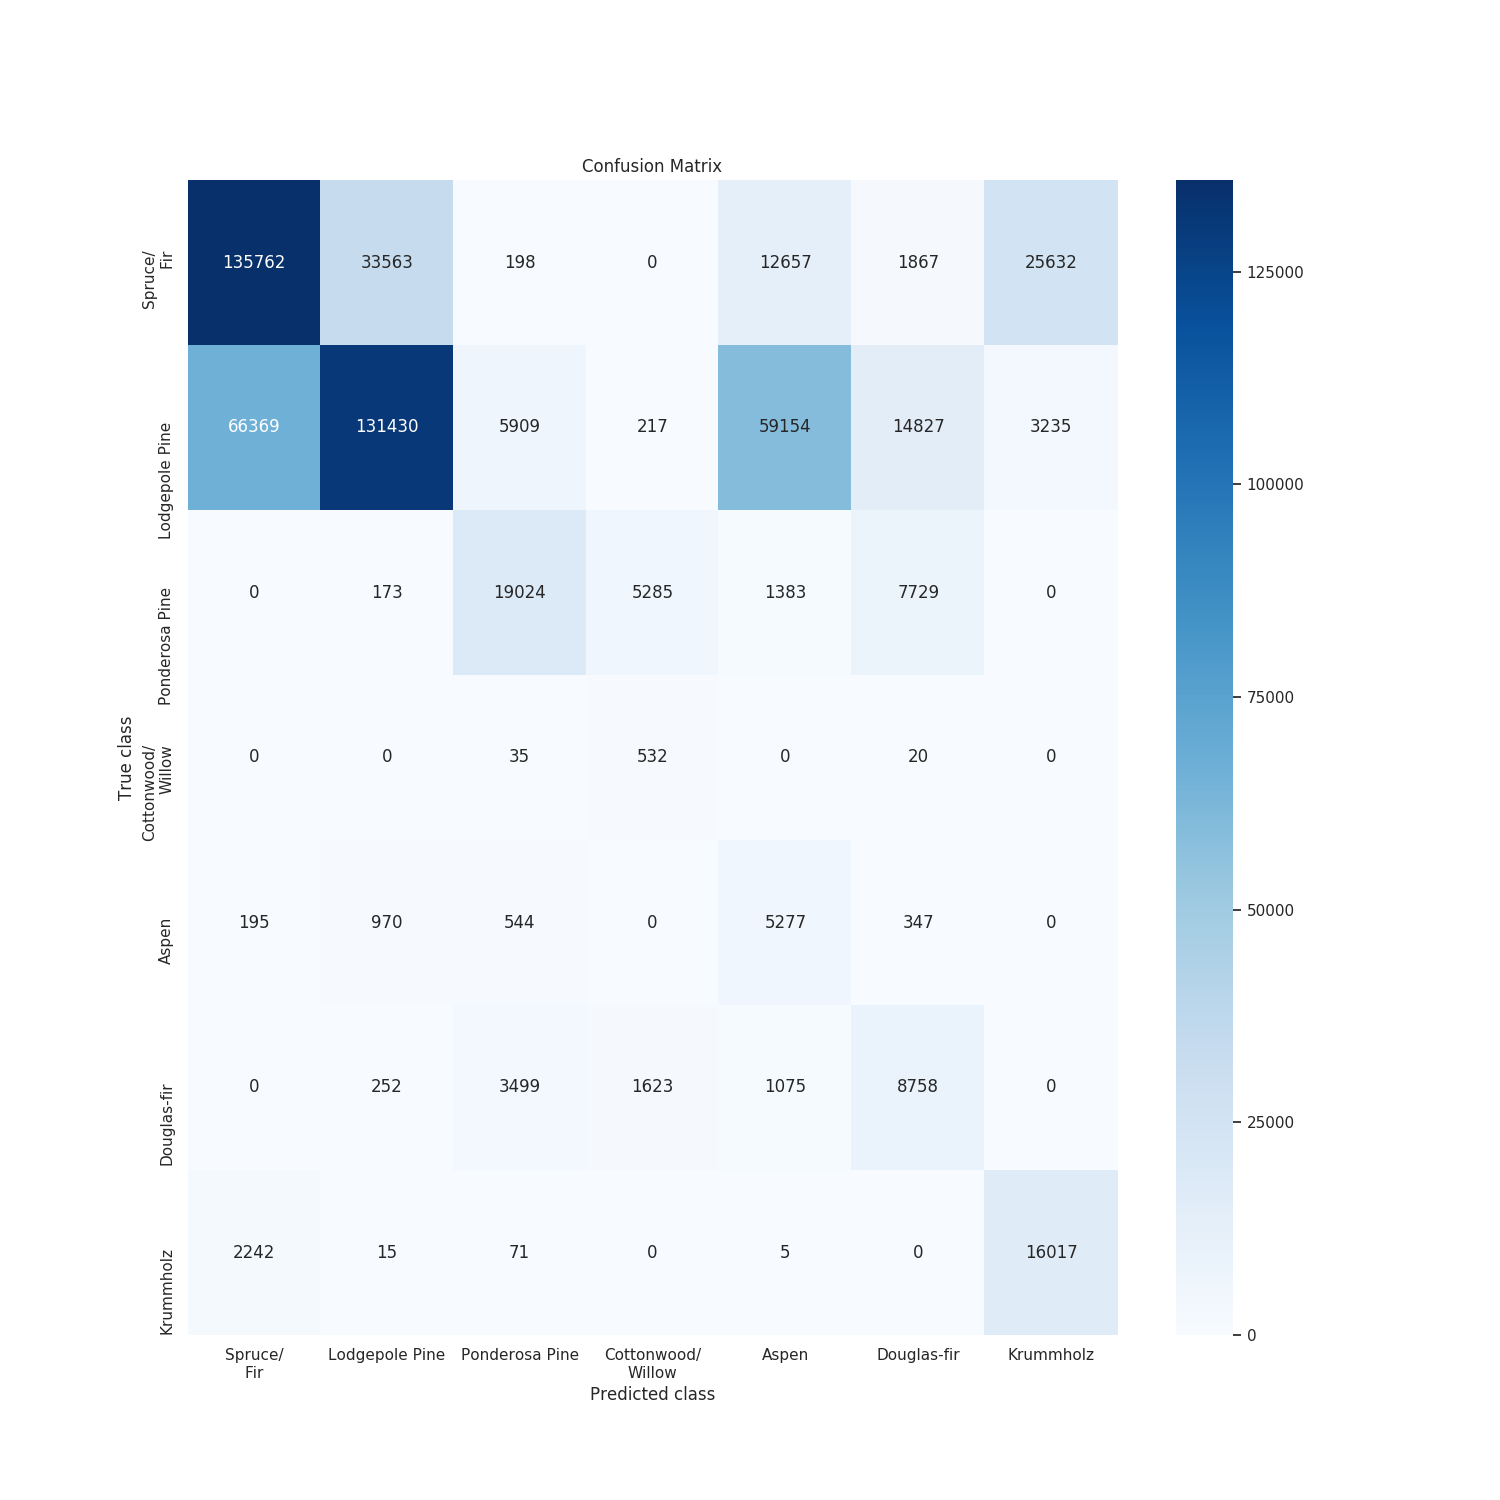
\includegraphics[width=\textwidth]{./TeX_files/img/confmatheatmap.png}
\caption{Heat-map rendering of the confusion matrix.}
\label{fig:confmatheatmap}
\end{figure}
% La tabella va aggiustata come in 
% https://tex.stackexchange.com/questions/2441/how-to-add-a-forced-line-break-inside-a-table-cell
\begin{table}
\centering
\resizebox{0.9\textwidth}{!}{
\begin{tabular}{ccccc}
& precision & recall & f1-score & support \\ \hline
Spruce/Fir        & 0.6637    & 0.6475 & 0.6555   & 209679  \\ \hline
Lodgepole Pine    & 0.7898    & 0.4675 & 0.5873   & 281141  \\ \hline
Ponderosa Pine    & 0.6497    & 0.5663 & 0.6051   & 33594   \\ \hline
Cottonwood/Willow & 0.0695    & 0.9063 & 0.1291   & 587     \\ \hline
Aspen             & 0.0663    & 0.7196 & 0.1215   & 7333    \\ \hline
Douglas-fir       & 0.2611    & 0.5759 & 0.3593   & 15207   \\ \hline
Krummholz         & 0.3569    & 0.8729 & 0.5066   & 18350   \\ \hline
weighted avg      & 0.6964    & 0.5598 & 0.5984   & 565891  \\ \hline
test set accuracy          & 0.5598    & 0.5598 & 0.5598   & 0.5598  \\ \hline
\end{tabular}
}
\caption{Precision, recall, f1-score summary table. Support indicates the number of occurrences of each particular class in the true responses (for the test set). Weighted avg is the per metric weighted average where the weights correspond to the support of that class.}
\label{tab:classificationrep}
\end{table}
\section{Our model}